\documentclass{standalone}
\usepackage{tikz}
\usetikzlibrary{shapes.geometric, shapes.misc, arrows}
\usetikzlibrary{positioning}
\usetikzlibrary{spy}
\usepackage[europeanresistors]{circuitikz}
\begin{document}
	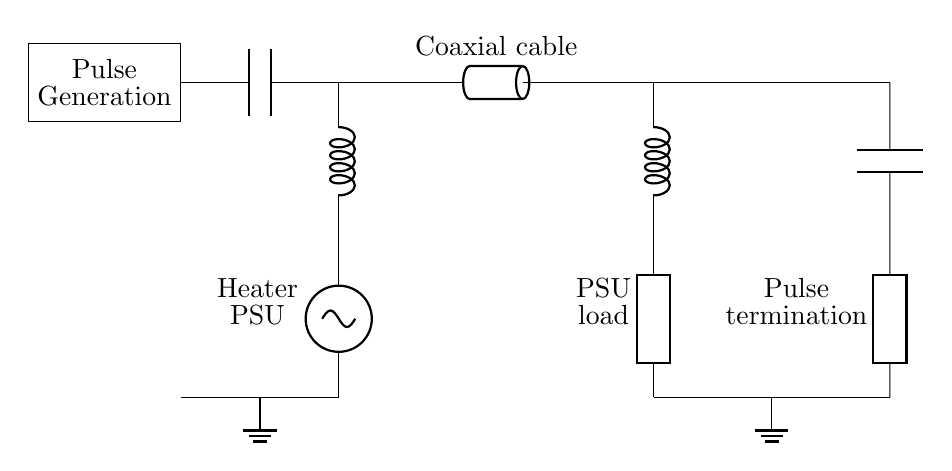
\begin{tikzpicture}

			\node (pulse_gen) [rectangle, draw, minimum size=1cm] {\shortstack{Pulse\\Generation}};
%			to[node, t=\shortstack{Pulse\\Gen.}] ++(1,0)
%			to[twoport, t=\shortstack{Pulse\\Gen.}] ++(1,0)
		\draw (pulse_gen.east)
			to[C] ++(2,0) coordinate (heater_top);

		\draw (heater_top)
			to[L] ++(0,-2)
			to[sV, l_=\shortstack{Heater\\PSU}] ++(0,-2)
			coordinate(heater_btm)
			to[short] ++(-1,0)
			node[ground] {}
			to[short] ++(-1,0);
			
		\draw (heater_top)
			to[TL, l^=Coaxial cable]  ++(4,0)
			coordinate (load_top);
			
		\draw (load_top)
		to[L] ++(0,-2)
		to[R, l_=\shortstack{PSU\\load}] ++(0,-2)
		coordinate(load_btm);
		
		\draw (load_top)
		to[short] ++(3,0)
		coordinate (pulse_term_top);
		
		\draw (pulse_term_top)
		to[C] ++(0,-2)
		to[R, l_=\shortstack{Pulse\\termination}] ++(0,-2)
		coordinate(pulse_term_btm);
		
		\draw (load_btm)
		to[short] ++(1.5,0)
		coordinate[ground]
		to[short] ++(1.5,0);
			
	\end{tikzpicture}
\end{document}
